\documentclass[letterpaper]{article}
\usepackage[submission]{aaai2026}
\usepackage{times}
\usepackage{helvet}
\usepackage{courier}
\usepackage[hyphens]{url}
\usepackage{graphicx}
\urlstyle{rm}
\def\UrlFont{\rm}
\usepackage{natbib}
\usepackage{caption}
\frenchspacing
\setlength{\pdfpagewidth}{8.5in}
\setlength{\pdfpageheight}{11in}
\usepackage{amsmath}
\usepackage{amssymb}
\usepackage{booktabs}
\usepackage{kotex}
\setmainhangulfont{Noto Serif CJK KR}
\setsanshangulfont{Noto Sans CJK KR}
\XeTeXlinebreaklocale ""
\setcounter{secnumdepth}{2}
\renewcommand{\tablename}{표}
\renewcommand{\figurename}{그림}
\renewcommand{\refname}{참고문헌}
\renewenvironment{abstract}{\centerline{\bf 초록}\vspace{0.5ex}\setlength{\leftmargini}{10pt}\begin{quote}\small}{\par\end{quote}\vskip 1ex}

\title{생산계획 기반 베이지안 어텐션 전달모형을 이용한\\제조공장 일전 전력 예측과 피크 저감 생산 재배치}

\begin{document}
\maketitle

\begin{abstract}
제조공장의 전력 수요는 설비 가동 일정에 따라 크게 달라지며, 최대수요전력은 12개월 래칫 규정을 통해 이후 1년간의 기본요금을 결정한다. 본 연구는 베이지안 어텐션 전달모형(Bayesian Attention Transfer, BAT)을 제안한다. BAT는 시간별 생산계획에서 하루 96개 15분 슬롯의 전력 곡선을 예측하고 예측 모델의 사후분포를 생산 재배치 의사결정에 연결한다. 모형은 가동유형별 기본곡선과 희소 국소 어텐션으로 구성되며 이 어텐션에서 전력 슬롯은 인접 생산 시각을 참조한다. 어텐션의 폭·모양·지연과 생산 이득은 Gibbs 표집과 Metropolis 갱신으로 추정한다. 실제 관측일이 65일에 불과한 KAMP 자원 최적화 데이터셋에서 BAT는 7–8월 검증 구간 56일 동안 생산계획을 입력받는 LightGBM보다 MAE를 33\% 줄였고(7.82 대 11.64 kW), CRPS와 일 피크 오차도 개선하였다. 9월 봉인 시험 구간에서는 두 모델이 대등하였다. 추정된 전달구조에서 전력 상승은 생산계획보다 0–2시간 이르다. 분포 기반 시간대 이동에는 이 구조와 함께 한국전력 산업용 요금과 인건비 할증을 반영하였다. 그 결과 검증 가동일 38일 중 20일에서 일 피크를 중앙값 3.4 kW 낮추는 계획이 권고되었다.
\end{abstract}

\section{서론}

\subsection{동기}
제조기업의 전기요금은 사용량에 비례하는 전력량요금과 최대수요전력에 따라 정해지는 기본요금으로 나뉜다. 한국전력 산업용(을) 요금에서 기본요금은 직전 12개월 가운데 여름·겨울철 최대수요전력으로 결정되므로, 한 번의 피크가 이후 1년의 비용을 좌우한다. 피크는 생산 일정에서 비롯되는데 본 연구 대상 공장에서 일 최대전력과 하루 생산 시간 수의 상관계수는 0.78이지만 일 최대전력과 기온의 상관계수는 $-0.005$에 그친다. 따라서 피크를 관리하려면 생산계획이 전력 곡선을 어떻게 만드는지 정량화하고, 이를 바탕으로 생산 시점을 조정할 수 있어야 한다.

\subsection{기존 접근의 한계}
제조공장 전력 예측 연구는 주로 일 단위 작업량과 기상을 입력으로 삼으며 시간별 생산계획은 실무에서 드물다는 이유로 다루지 않는다 \citep{kim2023c2transformer}. 트랜스포머 계열 모델은 수백 일 규모의 소표본 시계열에서 단순 선형 분해 모델보다 성능이 낮다는 보고가 있다 \citep{zeng2023dlinear}. 기울기 부스팅 모델은 점예측이 강하지만 입력과 출력 사이의 전달구조를 드러내지 않고, 예측구간이 좁아지는 경향이 있다. 예측과 의사결정을 잇는 연구 흐름 \citep{mandi2024dfl}은 대체로 가격 예측과 저장장치 운영에 집중되어 있다. 예측 불확실성은 생산 일정 조정의 근거가 되지만 이를 의사결정 규칙에 직접 반영한 사례는 찾기 어렵다. 마지막으로 공개 제조 데이터에는 증강을 위해 복사된 날이 섞여 있어, 이를 그대로 학습하면 실제 표본 크기가 과대평가되고 지연 특성이 오염된다.

\subsection{기여}
\begin{itemize}
\item 시간별 생산계획을 입력으로 받는 베이지안 어텐션 전달모형을 제안한다. 베이지안 분포지연모형 \citep{welty2009bdlm}의 지연 커널을 희소 어텐션 \citep{martins2016sparsemax} 형태로 구성하고, 어텐션 파라미터의 사후분포를 추정한다 \citep{fan2020bam}. 생산 이득을 양수로 제한하여 생산량이 늘 때 예측 전력이 줄지 않도록 한다.
\item 예측 사후분포에서 슬롯 간 상관을 보존하는 경로를 생성하여 점예측, 분위수, 일 피크, 피크 초과 확률을 하나의 분포에서 일관되게 산출한다.
\item 시작 시각과 시간당 생산량의 분포를 과거 생산계획에서 추정하여 현실적인 시간대 이동 후보를 만들고 요금 시간대·래칫·인건비 할증 규칙 아래에서 사후확률 기준을 충족하는 계획만 권고한다.
\item 증강 복사일 판정, 잠재 날짜효과가 수준 정보를 흡수하는 현상, 전력이 생산계획을 선행하는 지연 구조 등 데이터에서 확인한 사실을 절제 실험과 함께 제시한다.
\end{itemize}

\section{방법론}

\subsection{문제 정의}
날짜 $d$의 00시에 당일 전력 $y_{d,t}$ $(t=1,\dots,96)$를 예측한다. 입력은 당일 시간별 생산계획 $q_{d,h}$ $(h=0,\dots,23)$, 요일·공휴일·가동 여부, 그리고 $d$ 이전 날짜의 관측 전력이다. 생산계획에서 하루 생산 시간 수를 세어 가동유형 $k\in\{0,1,2,3\}$(0시간, 1–12시간, 13–19시간, 20시간 이상)을 정한다.

\subsection{베이지안 어텐션 전달모형}
BAT의 평균 구조는 다음과 같다.
\begin{equation}
y_{d,t} = \mu_{k,t} + \gamma_k\, r_{d,t} + \sum_{c} w_{c,k} \sum_{h} \alpha_{t,h}(\theta_k)\, x_c(q_{d,h}) + \varepsilon_{d,t}
\end{equation}
$\mu_{k,t}$는 가동유형별 기본곡선으로, 순환 2차 확률보행 사전분포 \citep{rue2005gmrf}로 평활한다. $r_{d,t}$는 가동 여부와 날짜유형이 같은 가장 최근 완전 관측일의 전력 곡선이다. 생산 채널 $x_c$는 가동 여부 $\mathbb{1}[q>0]$와 로그 생산량 $\log(1+q)/\log(1+q_{\max})$의 두 가지이다. 전력은 생산량보다 가동 여부에 더 민감하므로 두 채널을 분리한다. 생산 이득은 $w_{c,k}=\exp(\omega_{c,k})>0$으로 매개화한다.

어텐션 가중치는 전력 슬롯 $t$와 생산 시각 $h$ 사이의 시간 거리 $\Delta_{t,h}$로 일반화 가우시안 점수를 구하고 이를 sparsemax로 정규화한 값이다.
\begin{equation}
\alpha_{t,h}(\theta) = \operatorname{sparsemax}_h\!\left(-\frac{|\Delta_{t,h}-c|^{\beta}}{\sigma}\right)
\end{equation}
폭 $\sigma$, 모양 $\beta$, 지연 $c$만 학습하므로 어텐션의 학습 파라미터는 가동유형당 3개이다. sparsemax는 먼 시각의 가중치를 정확히 0으로 만들어, 주변 시간에 생산이 없으면 전달항이 사라지고 예측이 기본곡선으로 돌아가게 한다. $\alpha\ge 0$이고 $w>0$이므로 예측 전력은 생산계획에 대해 단조 증가한다.

\subsection{사후 추론}
오차 $\varepsilon$에는 Laplace 분포를 두고, 정규–지수 척도 혼합 표현 \citep{park2008blasso,kozumi2011bqr}으로 조건부 켤레성을 확보한다. 표집은 다음 순서로 반복한다. (i) 혼합 척도의 역수를 역가우시안 분포에서 뽑는다. (ii) 기본곡선과 $\gamma$를 가중 정규방정식에서 한 번에 뽑는다. (iii) 가동유형별 $(\log\sigma,\log\beta,c,\omega)$를 랜덤워크 Metropolis로 갱신한다. (iv) 평활 분산을 역감마 분포에서 뽑는다. 학습 우도에는 반감기 30일의 시간 가중을 적용한다. 계절에 따라 전력 수준이 이동하므로, 모든 날을 같은 비중으로 두면 최근 수준을 따라가지 못하고 잡음 분산을 과대추정한다. 2,000회 반복 가운데 앞의 1,000회를 버린다.

\subsection{예측분포}
사후 표본 $s$마다 평균 곡선을 계산하고, 날짜 공통 이동 $u\sim\mathcal{N}(0,\sigma_u^2)$와 하루 안 AR(1) 잡음 $e_t=\rho e_{t-1}+\eta_t$ $(\eta_t\sim\text{Laplace})$를 더해 경로를 만든다. $\rho$와 잡음 척도는 학습 잔차에서 표본마다 추정한다. 학습 잔차에서 추정한 인접 슬롯 자기상관이 0.74–0.82로 높으므로, 슬롯별로 독립인 잡음을 쓰면 하루 최댓값이 체계적으로 부풀려진다. 점예측은 경로의 중앙값이며, 분위수·일 최대·피크 초과 확률은 같은 경로에서 계산한다. 피크 초과 확률은 내부 보정일에서 적합한 Platt 보정 \citep{platt1999probabilistic}을 거친다.

\subsection{사후 기반 생산 재배치}
첫째 재배치 전략은 가동 시각을 고정하고 생산량만 옮긴다. 예측 곡선이 생산계획에 대해 미분 가능하므로 재배치 계획 $q'$를 다음 문제로 구한다.
\begin{equation}
\min_{q'}\; \lambda_D\,\mathrm{LSE}_\tau\!\left(\hat y(q')_{\mathcal{D}}\right) + \sum_t 0.25\, p_t\, \hat y_t(q') + \lambda_L \sum_h \ell_h q'_h
\end{equation}
$\mathcal{D}$는 기본요금 산정 대상 시간대(중간·최대부하), $p_t$는 시간대별 전력량 단가, $\ell_h$는 인건비 할증 배수이다. 제약은 일 총생산 보존, 기존 가동 구간 안에서만 이동, 시간당 상한(학습기간 시간대별 95분위), 이동량 $\le \rho_{\mathrm{m}}\sum_h q_h$이다. 매 경사 단계 뒤에는 Dykstra 교대 투영으로 박스·초평면 제약과 $L_1$ 이동량 제약의 교집합에 투영한다.

둘째 전략인 분포 기반 시간대 이동은 가동 시각 자체를 옮긴다. 학습기간의 생산계획에서 두 분포를 추정한다. 가동 블록의 시작 시각은 가동유형별 범주형 분포로 두고 Dirichlet(0.5) 사전분포를 더한다. 시작 시각은 거의 모두 0, 1, 7, 8시이다. 가동 시각의 시간당 생산량은 주간(07–20시)과 야간으로 나누어 Gamma 분포로 적합한다. Gamma의 Kolmogorov–Smirnov 통계량은 0.043으로 로그정규(0.095)와 지수 분포(0.133)보다 작았다. 주간 생산량 중앙값은 1,032, 야간은 85–120으로 약 10배 차이가 난다. 후보 계획 (i)은 가동 블록 전체를 1–2시간 이동하되 새 시작 시각의 사후예측확률이 5\% 이상이어야 한다. 후보 (ii)는 단가가 높은 시각의 생산을 단가가 낮은 인접 가동 시각으로 옮기되 옮긴 뒤의 생산량이 해당 시간대 Gamma 분포의 95분위를 넘지 않아야 한다. 계획과 실제 생산의 차이는 시각별 곱셈 오차 $\mathrm{LogNormal}(0,\sigma^2)$로 두고, 계획 자료가 없으므로 $\sigma\in\{0.05,0.1,0.2\}$로 민감도를 확인한다.

두 전략 모두 사후 표본(시간대 이동은 실행 오차 표본을 함께 사용)마다 새 계획의 일 피크를 계산하여, $P(\text{피크 감소})\ge 0.95$인 계획만 권고한다. 여러 후보가 기준을 통과하면 기대 요금이 가장 낮은 계획을 고른다.

\section{실험 설정}

\subsection{데이터}
KAMP 자원 최적화 AI 데이터셋(\texttt{okm\_augumented\_2021.csv})을 사용한다(변수 구성은 표~\ref{tab:data}).

\begin{table}[t]
\centering
\footnotesize
\setlength{\tabcolsep}{3pt}
\begin{tabular}{@{}lll@{}}
\toprule
변수 & 단위·범위 & 사용 \\
\midrule
날짜, 시간 & 2021.1.1–9.14, 1시간 & 색인 \\
전력(15분 단위) & kW, 19–222 & 목표 \\
생산량 & 개/시간 & 생산계획 입력 \\
기상 4종$^{a}$ & 관측값 & 미사용 \\
전기요금(계절) & 원/kWh & 계절 지시만 \\
인건비 & 할증 배수 1.0/1.5 & 재배치 제약 \\
공장인원, 평균 & 파생값 & 누수로 제거 \\
\midrule
원자료 / 15분 변환 & \multicolumn{2}{l}{6,168행 / 24,672슬롯} \\
기간 / 가동일 / 공휴일 & \multicolumn{2}{l}{257일 / 195일 / 8일} \\
복사일(완전·편집) & \multicolumn{2}{l}{122일 (115·7)} \\
\bottomrule
\end{tabular}
\caption{데이터 구성. $^{a}$기온·풍속·습도·강수량. 일 최대전력과 기온의 상관계수는 $-0.005$이다.}
\label{tab:data}
\end{table}

\subsection{전처리 전략}
시간 단위 원자료를 15분 슬롯으로 펼치고, 구간 시작 시각을 슬롯 라벨로 쓴다. 전처리의 핵심은 증강 복사일의 판정이다. 115쌍의 날은 96개 슬롯 전력이 소수점까지 일치하지만, 같은 쌍의 기온과 습도는 한 쌍도 일치하지 않는다. 복사가 없는 7–8월의 실제 가동일 861쌍은 같은 값을 가진 슬롯이 최대 25개이다. 이에 따라 전력 곡선만 복사된 날로 판정하고, 그룹별 원본 하나만 남긴 채 목표와 기준일 참조에서 마스킹한다. 가동구간에서 20개 이상의 슬롯이 일치하는 편집 복사 7일도 같은 방식으로 처리한다. 복사일 122일 중 121일이 1–6월에 있어, 첫 번째 검증 fold의 학습기간 186일 가운데 실제 관측일은 65일이다. 전력 0인 74개 슬롯은 계측 손실로 보고 결측 처리하며, 시각 정보가 소실된 7월 13일과 15일의 목표도 마스킹한다.

복사일 판정이 평가에 주는 영향은 복사일을 포함한 자료에서 두 교차검증을 비교하여 확인하였다. 비교한 방식은 날짜 단위 무작위 5-fold와 복사 그룹 전체를 한 번에 제외하는 LOEO(leave-one-event-out, 126개 그룹)이다. 같은 날짜끼리 짝지어 비교하면 M2의 MAE는 무작위 5-fold에서 14.91 kW, LOEO에서 16.64 kW로 차이가 $-1.73$ kW(95\% 신뢰구간 $[-3.63,-0.04]$)였다. 시험일의 복사본이 학습에 섞이면 M2의 성능이 약 10\% 과대평가된다. BAT는 16.37 kW와 16.32 kW로 차이가 없었다($+0.05$, $[-0.22,0.42]$). 이 결과를 근거로 복사일을 마스킹하고 시간 순서를 지키는 fold로 모델을 평가한다(그림~\ref{fig:loeo}).

\begin{figure}[t]
\centering
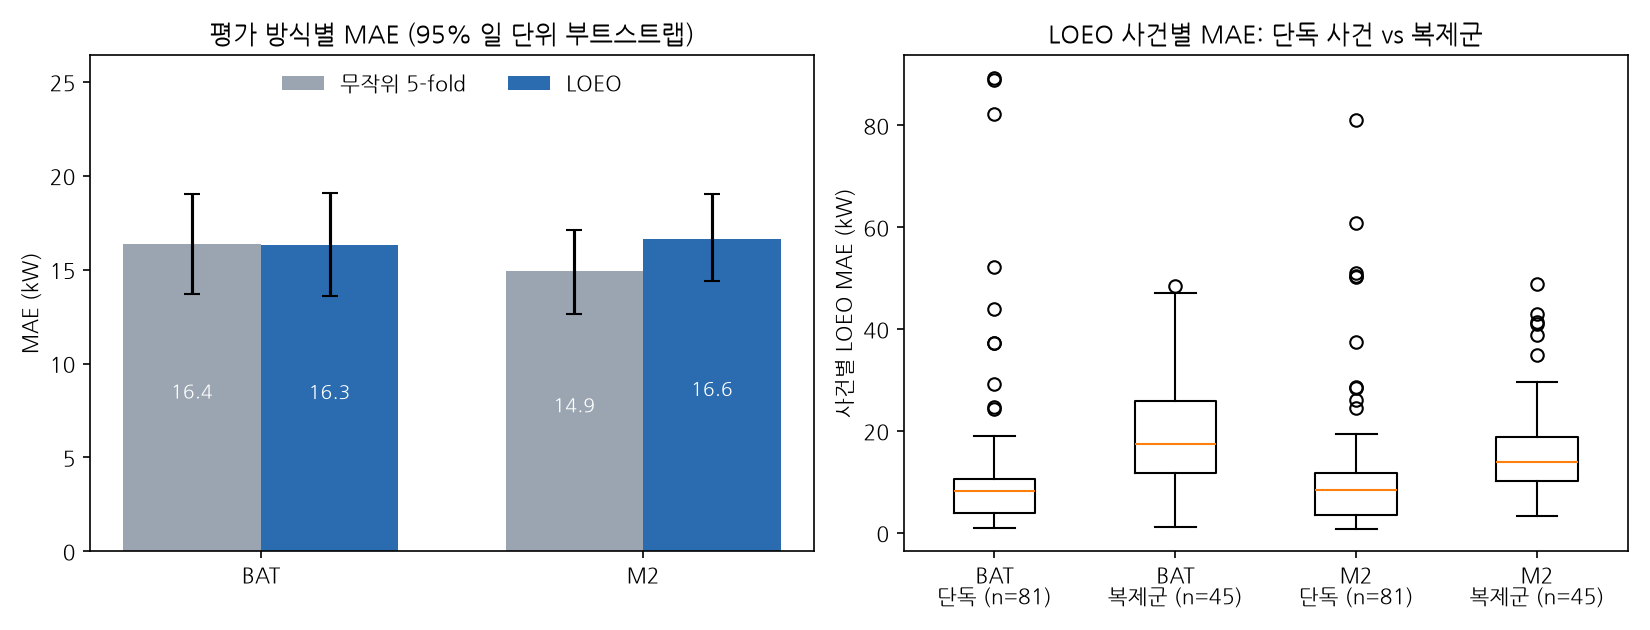
\includegraphics[width=\columnwidth]{figs/leakage_gap.png}
\caption{복사일을 포함한 자료의 교차검증 비교. 왼쪽: 무작위 5-fold와 LOEO의 MAE(95\% 부트스트랩 구간). 오른쪽: LOEO 그룹별 MAE, 단독일과 복사 그룹 구분.}
\label{fig:loeo}
\end{figure}

\subsection{검증 설계와 비교 모델}
시간 순서를 지키는 4개 검증 fold(7월 7일–8월 31일, fold당 14일)에서 모델을 선택하고, 9월 1–14일을 봉인 시험 구간으로 둔다. 각 fold의 학습기간은 검증 구간 직전까지 확장되며, 모든 모델은 날짜 $d$를 예측할 때 $d$ 이후의 전력값을 보지 못하도록 감싼다. 비교 모델 B0는 지난주 같은 요일 곡선을 그대로 쓰고 M2는 생산계획·달력·지연 특성을 입력으로 하는 LightGBM 분위수 모델이다 \citep{ke2017lightgbm}. 평가 지표는 MAE, 분위수 기반 CRPS \citep{gneiting2007scoring}, 일 최대전력 오차, 예측구간 적중률이다. 피크 초과 분류는 학습기간 일 최대전력의 50·75·90분위($C_{50},C_{75},C_{90}$)를 넘는 날을 사건으로 두고, 보조 지표로서 F1 점수를 보고한다. 두 모델의 차이는 날짜 단위 짝짓기 부트스트랩(2,000회)으로 검정한다.

\section{결과}

\subsection{예측 성능}
검증 구간에서 BAT의 MAE는 M2보다 3.81 kW 낮았으며(표~\ref{tab:main}) 95\% 신뢰구간은 $[-6.35,-1.62]$였다. CRPS 차이의 신뢰구간 $[-3.87,-0.31]$도 0을 포함하지 않는다. fold별로 보면 4개 가운데 3개에서 BAT의 MAE가 M2보다 낮았다. 예측구간의 80\% 적중률은 BAT가 0.90, M2가 0.62로, M2는 불확실성을 과소평가하였다. 봉인 시험 구간에서는 MAE가 6.82와 6.60, RMSE가 9.53과 9.75로 두 모델이 비슷한 수준이었다(그림~\ref{fig:test}). 그림~\ref{fig:val}의 f1 예시(7월 12일)에서 M2는 생산이 없는 새벽 시각의 전력을 약 55 kW로 예측했지만 BAT는 대기부하 수준(약 23 kW)에 근접했다.

\begin{figure*}[t]
\centering
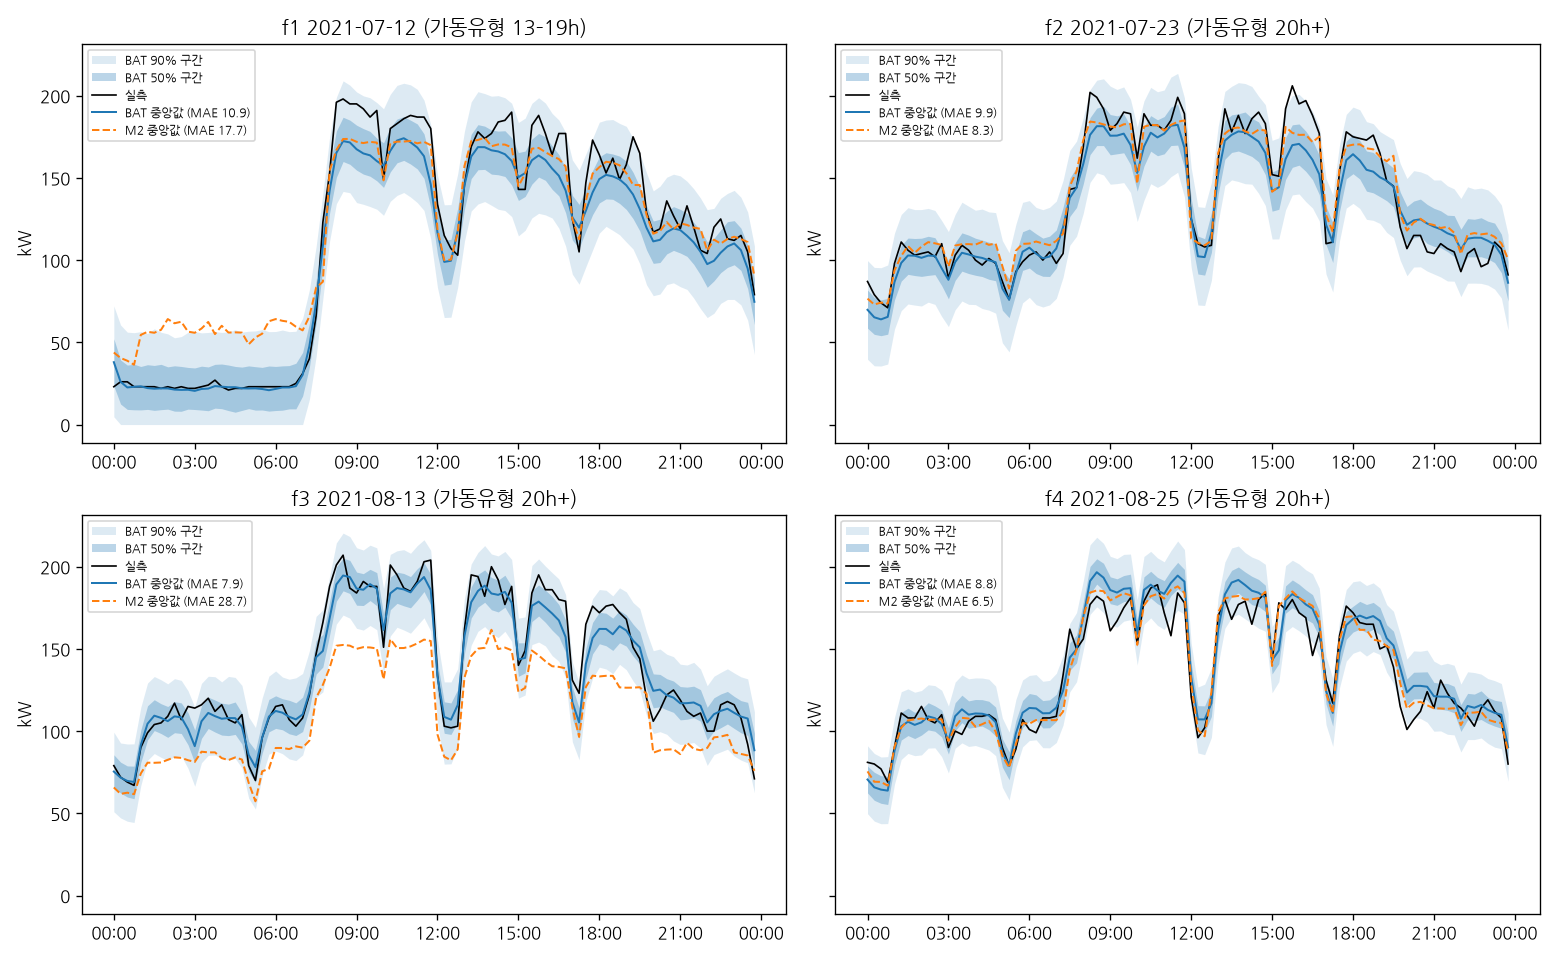
\includegraphics[width=0.9\textwidth]{figs/forecast_val.png}
\caption{검증 fold별 대표일(일 MAE가 fold 중앙값에 가장 가까운 가동일)의 실측, BAT 중앙값과 50·90\% 예측구간, M2 중앙값.}
\label{fig:val}
\end{figure*}

\begin{figure*}[t]
\centering
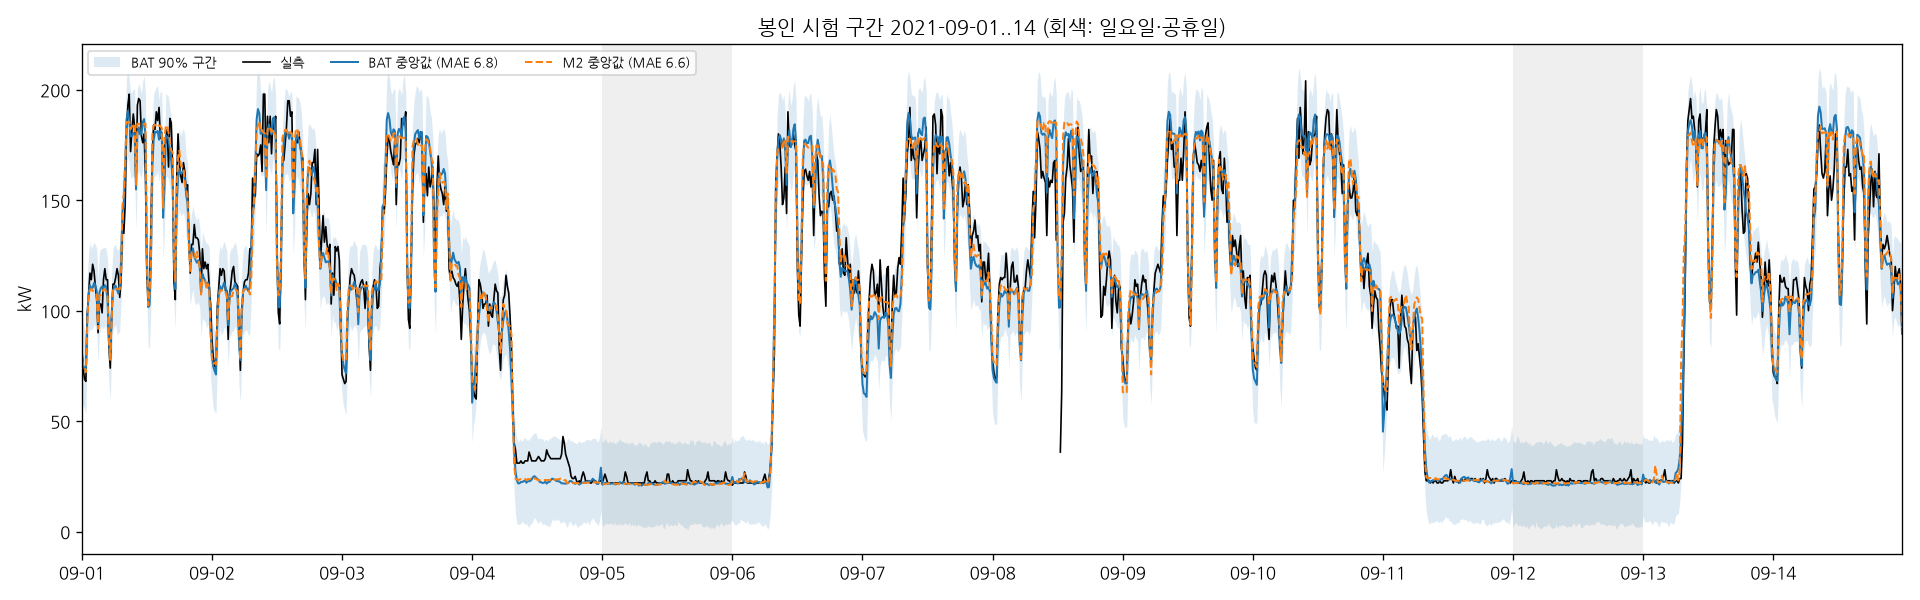
\includegraphics[width=\textwidth]{figs/forecast_test.png}
\caption{봉인 시험 구간(2021년 9월 1–14일)의 실측, BAT 중앙값과 90\% 예측구간, M2 중앙값. 회색은 일요일이다.}
\label{fig:test}
\end{figure*}


\begin{table}[t]
\centering
\small
\begin{tabular}{@{}llccc@{}}
\toprule
구간 & 지표 & BAT & M2 & B0 \\
\midrule
검증 & MAE & \textbf{7.82} & 11.64 & 26.84 \\
(56일) & CRPS & \textbf{6.99} & 8.96 & -- \\
 & 일 피크 MAE & \textbf{14.5} & 17.0 & 42.2 \\
 & 80\% 구간 적중 & 0.90 & 0.62 & -- \\
\midrule
시험 & MAE & 6.82 & \textbf{6.60} & 7.88 \\
(14일) & RMSE & \textbf{9.53} & 9.75 & 11.18 \\
 & CRPS & 5.51 & \textbf{5.03} & -- \\
 & 일 피크 MAE & 7.98 & \textbf{5.53} & 7.00 \\
\bottomrule
\end{tabular}
\caption{예측 성능(단위 kW, CRPS와 적중률 제외).}
\label{tab:main}
\end{table}

\subsection{절제 실험}
설계 요소별 기여는 표~\ref{tab:ablation}과 같다. 날짜별 잠재효과를 평균식에 넣으면, 학습 중에는 이 효과가 기준일의 수준 정보를 흡수하고 예측 시점에는 0으로 두게 되어 첫 fold의 MAE가 19.0으로 나빠졌다. 반감기 가중은 계절 수준 변화를 반영하여 MAE를 9.9에서 7.8로 낮췄다. 슬롯 독립 잡음을 AR(1) 잡음으로 바꾸자 일 피크 오차가 40.3에서 18.8로 줄었다. BAT 잔차에 3차 계층 보정을 더하면 오히려 MAE가 10.2로 나빠졌는데, 구조가 편향을 이미 제거하여 보정이 학습기간의 우연한 패턴을 학습했기 때문이다. 어텐션 전달항을 제거해도 MAE 차이는 0.7\%에 그치지만, 전달항이 없으면 같은 가동유형 안에서 예측이 생산 시각에 반응하지 않아 전달행렬과 재배치를 계산할 수 없다. 복사일을 포함해 학습하면 BAT의 MAE는 7.59로 거의 변하지 않았고, M2는 13.76으로 악화되었다.

\begin{table}[t]
\centering
\small
\begin{tabular}{@{}lcc@{}}
\toprule
설정 & 변경 전 & 변경 후 \\
\midrule
잠재 날짜효과 제거 (f1 MAE) & 19.0 & 13.1 \\
반감기 30일 가중 (MAE) & 9.9 & 7.8 \\
AR(1) 잡음 (일 피크 MAE) & 40.3 & 18.8 \\
3차 계층 보정 추가 (MAE) & 7.8 & 10.2 \\
어텐션 전달항 제거 (MAE)$^{b}$ & 9.93 & 9.99 \\
복사일 포함 학습, BAT (MAE) & 7.82 & 7.59 \\
복사일 포함 학습, M2 (MAE) & 11.64 & 13.76 \\
\bottomrule
\end{tabular}
\caption{절제 실험. 별도 표기가 없으면 검증 56일 전체 기준이다. $^{b}$반감기 가중을 적용하기 전 모델에서 측정하였다.}
\label{tab:ablation}
\end{table}

\subsection{오차와 피크 발생 조건}
가동유형과 해당 시각의 생산 여부로 나눈 영역별 MAE(표~\ref{tab:regime})에서 BAT는 24시간 가동일에서 생산이 없는 시각의 오차를 M2의 절반 이하로 낮췄다(8.0 대 18.7). 생산이 계획된 시각에서도 모든 가동유형에서 M2보다 오차가 작았다. 유일하게 M2보다 나빴던 영역은 12시간 이하 가동일의 비생산 시각(4.1 대 3.3)이다. 요금 시간대별로는 단가가 가장 높은 최대부하 시간대에서 예측 개선 폭이 가장 컸다(M2 대비 $-6.0$ kW).

\begin{table}[t]
\centering
\small
\begin{tabular}{@{}lrccc@{}}
\toprule
영역 & 슬롯 & BAT & M2 & B0 \\
\midrule
비가동일 & 1,394 & \textbf{1.7} & 4.4 & 34.3 \\
1–12h, 비생산 & 378 & 4.1 & \textbf{3.3} & 3.7 \\
1–12h, 생산 & 172 & \textbf{7.7} & 11.3 & 17.3 \\
13–19h, 비생산 & 268 & 9.3 & 15.4 & \textbf{6.2} \\
13–19h, 생산 & 500 & \textbf{16.1} & 18.0 & 28.2 \\
20h+, 비생산 & 108 & \textbf{8.0} & 18.7 & 29.2 \\
20h+, 생산 & 2,196 & \textbf{10.3} & 15.4 & 28.9 \\
\bottomrule
\end{tabular}
\caption{가동유형(하루 생산 시간 수)과 해당 시각 생산 여부별 MAE(kW).}
\label{tab:regime}
\end{table}

보조 지표인 피크 초과 분류에서 BAT의 F1 점수는 $C_{50}$, $C_{75}$, $C_{90}$에서 각각 0.95, 0.85, 0.54였고, M2는 0.93, 0.70, 0.32였다. 모든 날에 경보를 내는 기준 분류기의 F1 점수는 0.76, 0.58, 0.41이다. BAT는 세 기준 모두에서 이를 넘었지만, M2는 $C_{90}$에서 기준 분류기보다 낮았다. BAT의 $C_{90}$ 재현율은 0.77이고 정밀도는 0.42로, 놓친 피크는 3일, 오경보는 14일이다. 오경보는 주로 금요일과 생산 총량 상위 25\% 날에 발생했다.

\subsection{전달구조 해석}
13–19시간 가동유형의 어텐션 사후평균(그림~\ref{fig:attn})에서 가중치가 대각선에 집중되어 있어 전력은 인접 1–2시간의 생산계획에 반응한다. 지연 $c$의 사후 중앙값은 1–12시간, 13–19시간, 20시간 이상 가동유형에서 각각 $-0.60$, $-0.34$, $-2.30$시간이었다. 음의 지연은 전력이 생산계획보다 먼저 상승함을 뜻하며 설비 예열과 준비 가동의 영향으로 보인다. 가동 채널 이득 $w_{\mathrm{on}}$의 사후 중앙값은 각각 3.1, 13.2, 16.5 kW로, 가동 시간이 긴 유형일수록 커졌다.

\begin{figure}[t]
\centering
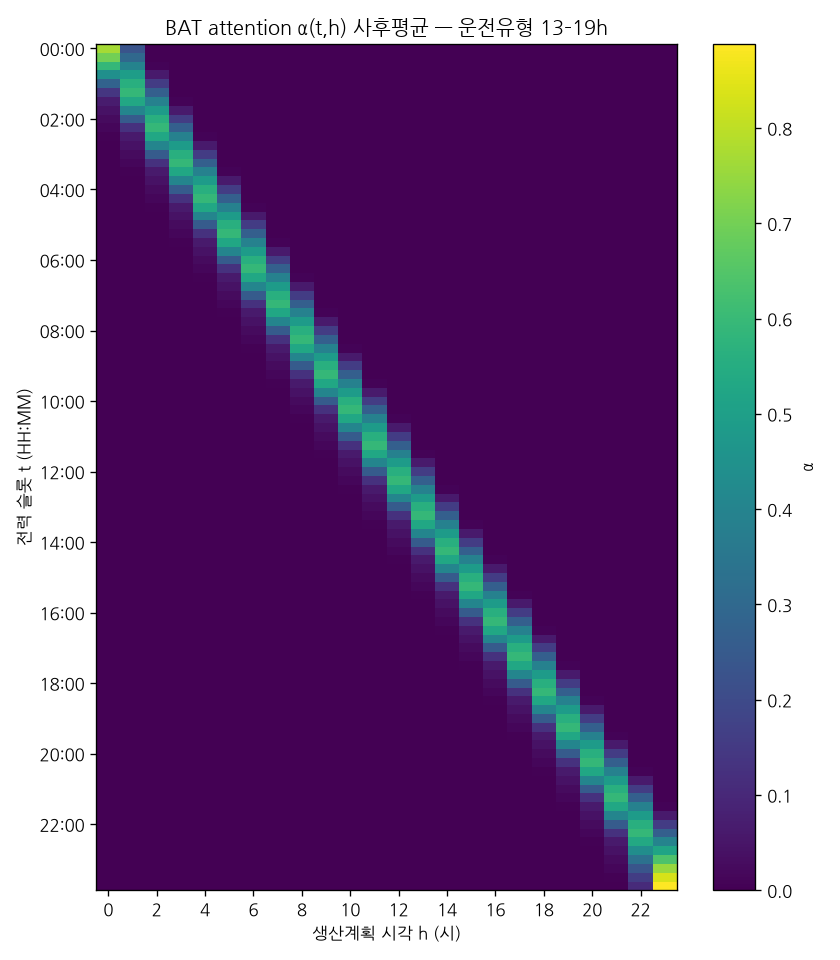
\includegraphics[width=0.92\columnwidth]{figs/attention_k2.png}
\caption{13–19시간 가동유형의 어텐션 가중치 $\alpha_{t,h}$ 사후평균. 세로축은 전력 슬롯, 가로축은 생산계획 시각이다.}
\label{fig:attn}
\end{figure}

\subsection{생산 재배치}
검증기간 가동일에서 두 재배치 전략을 비교하였다(표~\ref{tab:realloc}). 생산량 재배치(가동 시각 고정)는 39일 중 10일에서 기준을 통과했으나 권고일의 피크 감소 중앙값은 0.1 kW뿐이었다. 이 전략은 가동 시각을 바꾸지 않는데, 추정된 전달구조에서 전력은 생산량보다 가동 여부에 주로 반응하기 때문이다(가동 이득 13.2–16.5 kW).

분포 기반 시간대 이동에서는 38일 중 20일이 기준을 통과하였고 권고일의 피크 감소 중앙값은 3.4 kW, 최대 9.8 kW였다. 하루 요금 변화의 중앙값은 $-5{,}235$원이며, 가동일 22일을 기준으로 월 약 11.5만 원이다. 실행 오차를 $\sigma=0.05, 0.1, 0.2$로 바꾸어도 권고일은 20, 20, 19일로 거의 같았다. 권고된 계획 20건 가운데 19건은 11시의 생산을 12시로 옮겼다. 여름철 11시는 최대부하(191.1원/kWh), 12시는 중간부하(109.0원/kWh) 시간대이고 두 시각 모두 인건비 할증이 없어, 인건비 지수는 변하지 않았다. 이 20일 가운데 20시간 이상 가동일이 18일, 13–19시간 가동일이 2일이었다. 야간 생산량은 주간의 약 1/10 수준이므로 주간 생산을 야간으로 대량 이동하는 계획은 관측 지지 범위를 벗어나 후보에서 제외되었다.

7–8월의 래칫 바닥은 222 kW(7월 19일)이고 검증기간 일 피크는 187–201 kW이므로, 이 기간의 피크 감소는 기본요금을 낮추지 못하고 절감액은 대부분 전력량요금에서 나온다. 기본요금 절감은 당월 피크가 래칫 바닥을 넘는 달에만 실현된다.

\begin{table}[t]
\centering
\small
\setlength{\tabcolsep}{4pt}
\begin{tabular}{@{}lcc@{}}
\toprule
 & 생산량 재배치 & 시간대 이동 \\
\midrule
대상 가동일 & 39 & 38 \\
권고일 ($P\ge0.95$) & 10 & 20 \\
피크 감소 중앙값 (kW) & 0.1 & 3.4 \\
피크 감소 최댓값 (kW) & 1.0 & 9.8 \\
요금 변화 중앙값 (원/일) & $-1{,}194$ & $-5{,}235$ \\
인건비 지수 & 1.000 & 1.000 \\
\bottomrule
\end{tabular}
\caption{재배치 전략 비교(모델 기반 반사실 추정). 생산량 재배치는 $\rho_{\mathrm{m}}=0.2$, $\lambda_L=0$, 시간대 이동은 $\sigma=0.1$ 기준이다.}
\label{tab:realloc}
\end{table}

\section{한계와 논의}
첫째, 생산량은 데이터상 실적이며 본 연구는 이를 사전에 알려진 생산계획으로 가정하였다. 실제 계획과 실적의 차이가 크면 예측 성능이 낮아질 수 있다. 둘째, 검증 구간은 56일, 시험 구간은 14일로 짧다. 검증에서 확인된 우위가 봉인 시험 구간에서는 거의 나타나지 않았으며 시험 구간의 신뢰구간은 제시하지 못하였다. 셋째, 예측구간은 명목 수준보다 넓다(50\% 구간 적중률 0.74). 내부 보정일로 잡음 척도를 교정하는 방법을 시도했으나, 학습기간 말의 보정일이 검증기간보다 전력 변동이 작아 교정이 구간을 과도하게 좁혔으므로(80\% 구간 적중률 0.67) 보수적인 무교정 구간을 채택하였다. 넷째, 재배치 효과는 관측되지 않은 반사실이며, 모델이 학습한 생산–전력 관계가 재배치 이후에도 유지된다는 가정에 기댄다. 이 위험을 줄이기 위해 단조 제약, 관측 지지 범위, 사후확률 기준을 두었다. 권고된 계획 대부분은 12시 생산을 늘리는데, 이 시각이 휴게 시간이라면 교대 운영을 바꾸어야 적용할 수 있다. 다섯째, 단일 공장의 8개월 반 자료만 사용하였으므로 다른 공정과 계절로 일반화하려면 추가 검증이 필요하다. 시간별 생산계획이 기록되는 공장이라면 BAT의 구조, 즉 가동유형별 기본곡선과 생산 시각에 대한 희소 전달은 추가 설계 없이 쓸 수 있다.

\bibliography{refs}

\end{document}
